% \subsection {Algorithm Overview}

\begin{figure}
\begin{center}
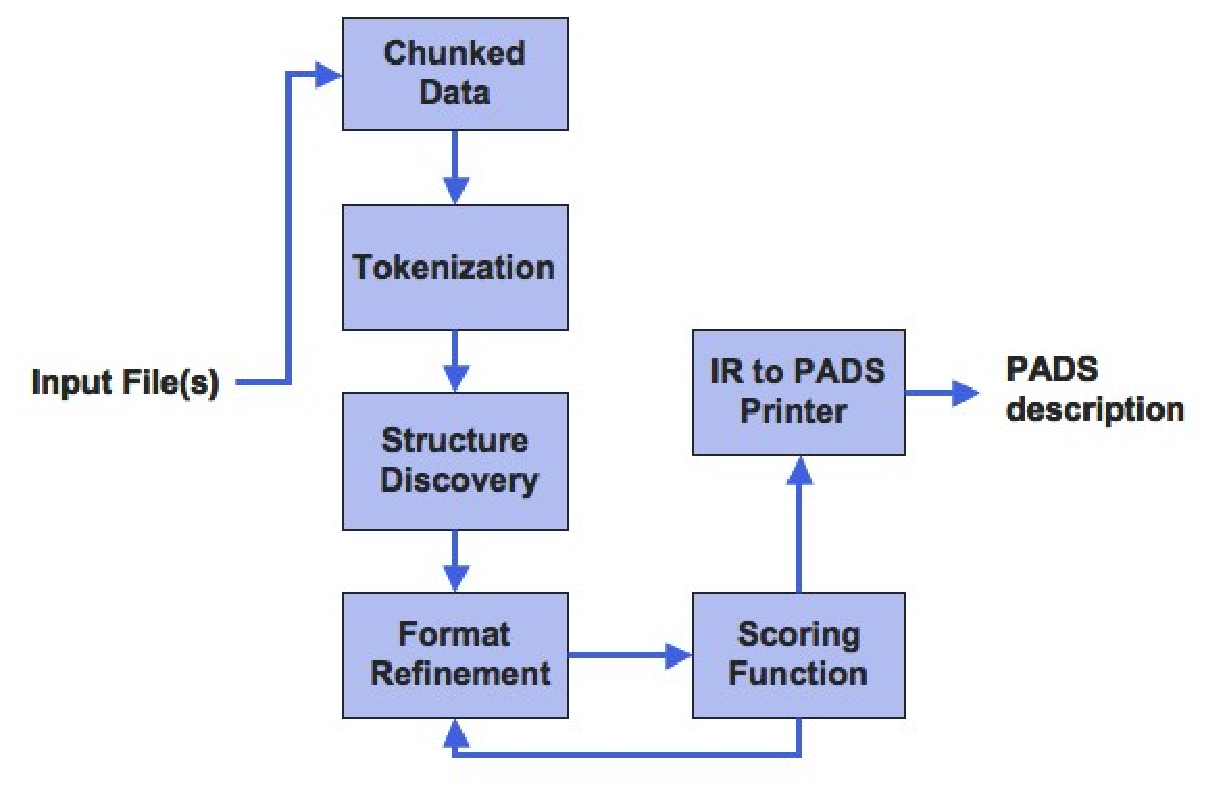
\epsfig{file=archi.eps, width=.9\columnwidth}
\caption{Architecture of the format inference engine}
\vspace*{-5mm}
\label{fig-archi}
\end{center}
\end{figure}

Figure \ref{fig-archi} gives an overview of our format inference
architecture. The input data, or ``training set,'' is first
``chunked'' into records where each record is a piece of recurrent
data such as a line, a paragraph, or a file (if the input consists of
multiple files).  The user specifies the unit of repetition when
invoking our learning tool.  Each record is then broken down into a
series of tokens where each token can be a punctuation symbol, a
number, a date, a time, or a number of other basic types.  Our
learning system has a basic tokenization scheme skewed toward systems
data, but users may specify a different scheme for their own domain
through a configuration file.  For example, computational biologists
may want to specify new base types for DNA strings or other common
recurring patterns.

In the structure discovery phase, we use a top-down, divide-and-conquer
scheme inspired in part by the work of Arasu on
information extraction from web pages~\cite{arasu+:sigmod03}. 
When a type constructor has been chosen, the data is partitioned accordingly
and the algorithm recursively analyzes subparts.  This
rough structure is represented in an intermediate representation (IR)
that has similar expressive power to the \pads{} language. 
The format refinement phase analyzes the IR produced by structure discovery
and repeatedly applies rewrite rules.  
In effect, this refinement phase is equivalent to a greedy, local search
procedure aimed at improving the quality of the inferred format.

\subsection {Chunking and Tokenization}

\begin{figure}
\begin{center}
\begin{tabular}{|l|l|}
\hline
Name   &  Description               \\ \hline\hline
Pint  &   Integer \\ 
Palpha & Alpha-numeric string including '$\_$' and '$-$' \\
Pip & IP address \\
Pemail & Email address \\
Pmac & Mac address \\
Pdate & Simple date format \\
Ptime & Simple time format \\
Ppath & File system path \\
Phostname & Hostname \\
Purl  & URL \\
PbXML & Beginning XML tag \\
PeXML & Ending XML tag \\
Pother & Punctuation character \\\hline
\end{tabular}

\caption{Basic token types in default configuration.}
\label{figure:base-types}
\end{center}
\end{figure}
 



    *  mention system parameterization for multiple tokenizations for different domains
    * mention current skew towards systems data
    * ignore problems in this section -- save that for discussion/future work section
    * mention stream of tokens generated for running example 

\subsection {Structure Discovery}

    *  role = quickly find a description in the "approximate area" of the correct description
    * explain structure of a generic "top-down" inference algorithm -- perhaps give pseudocode
    * explain our heuristics: generation of histograms, choice of struct, array, union, base type
    * grouping construct (introduce additional example as needed)
    * show (part of?) description of running example 

\subsection {Information-Theoretic Scoring}

    *  role = evaluate the "goodness" of the description relative to data
    * explain the information-theoretic principles
    * give the formulas 

\subsection {Structure Refinement}

    *  role = starting with the candidate structure, search for nearby descriptions that optimize an information theoretic scoring function
    * explain the 3 parts: value independent, value dependent, value independent
    * give (partial) list of rules used -- we need to work on notation for explaining these rules
    * illustrate several transformations using the running example
    * compare example after rewriting to the example from subsection 3.4 above
    * optional subsubsection: theory suggesting our algorithm is "correct" (we'd need a semantics for our IR then) 

\subsection {Finishing Up}

    * printing pads syntax and invoking toolchain
